\documentclass[12pt, twoside]{article}
\usepackage[letterpaper, margin=1in, head=30pt, headsep=0.1in]{geometry}
\usepackage[english]{babel}
\usepackage[utf8]{inputenc}
\usepackage{amsmath}
\usepackage{amsfonts}
\usepackage{amssymb}
\usepackage{tikz}
%\usetikzlibrary{quotes, angles}

\usepackage{graphicx}
\usepackage{enumitem}
\usepackage{multicol}

%\usepackage{pgfplots}
%\pgfplotsset{width=10cm,compat=1.9}
%\usepgfplotslibrary{statistics}
%\usepackage{pgfplotstable}
%\usepackage{tkz-fct}
%\usepackage{venndiagram}

\usepackage{fancyhdr}
\pagestyle{fancy}
\fancyhf{}
\renewcommand{\headrulewidth}{0pt} % disable the underline of the header
\raggedbottom
\newif\ifmeta
\metatrue %print standards and topics tags

\title{Math AI Worksheet Generator and Formative Assessment System}
\author{Chris Huson}
\date{August 2019}

\fancyhead[RE]{\thepage}
\fancyhead[RO]{\thepage \\ Name: \hspace{3cm}}
%\fancyhead[L]{BECA / Dr. Huson / 10th Grade Geometry\\* 7 June 2019}
%
%\begin{document}
%\subsubsection*{13.7 Homework: Cross sections, distance applications}
\fancyhead[L]{BECA / Dr. Huson / Geometry 02-Midpoint+distance\\* pset ID: 24}

\begin{document}

\subsubsection*{2-6DN-Distance+Perimeter.tex}
\begin{enumerate}
\item Given $\overleftrightarrow{PQ}$ as shown on the number line, with $P=-1$ and $Q=5.6$. \\[20pt] % Midpoint
    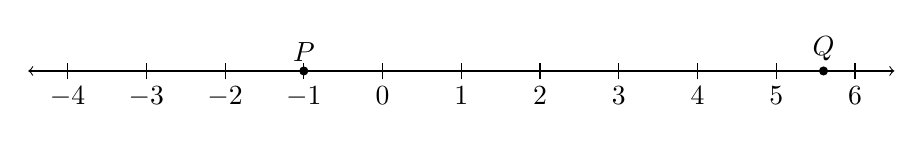
\begin{tikzpicture}
      \draw [<->] (-4.5,0)--(6.5,0);
      \foreach \x in {-4,...,6} %2 leading for diff!=1
        \draw[shift={(\x,0)},color=black] (0pt,-3pt) -- (0pt,3pt) node[below=5pt]  {$\x$};
        \draw [fill] (-1,0) circle [radius=0.05] node[above] {$P$};
        \draw [fill] (5.6,0) circle [radius=0.05] node[above] {$Q$};
    \end{tikzpicture} \\ \smallskip
    \begin{enumerate}
      \item What is the exact distance on the number line between the points $P$ and $Q$?  \vspace{2cm}
      \item Point $R$ is the midpoint of $\overline{PQ}$. Find $R$'s value. Mark it as a dot and label it on the number line $\overleftrightarrow{PQ}$.
    \end{enumerate}  \vspace{4cm}  

\item Find the perimeter of the shape shown below, given the side lengths marked (not drawn to scale). All angles are $90^\circ$. Completely mark the diagram with the two missing lengths and show an equation for $P$ as a sum of each side's length.
    \vspace{1cm} 
    \begin{flushleft}
    \begin{tikzpicture}
      \draw [-, thick] (0,0)--(5,0)--(5,2)--(3,2)--(3,6)--(0,6)--cycle;
      %\draw [fill] (0,0) circle [radius=0.05] node[left]{$A$};
      %\draw [fill] (7,0) circle [radius=0.05] node[right]{$B$};
      %\draw [fill] (7,2) circle [radius=0.05] node[right]{$C$};
      %\draw [fill] (0,2) circle [radius=0.05] node[left]{$D$};
      \node at (5.5, 1){4};
      \node at (4, 2.5){4};
      \node at (2.5, -0.5){10};
      \node at (-0.5, 3){12};
    \end{tikzpicture}
    \end{flushleft} \vspace{1cm}  

    \newpage

\item Given the diagram shown below. \vspace{0.25cm}
    \begin{enumerate}
      \item  Measure the angle $AEB$. $m \angle AEB = $ \rule{4cm}{0.15mm} \bigskip
      \item Name an angle that is complementary to $\angle CEB$: \rule{4cm}{0.15mm} \bigskip
      \item Name a pair of opposite rays: \rule{4cm}{0.15mm}
    \end{enumerate}
    %\vspace{1cm}
    \begin{center}
    \begin{tikzpicture}[scale=1.0, rotate=-20]
      \draw [->, thick] (0,0)--(70:5);
      \draw [<->, thick] (-6,0)--(5,0);
      \draw [->, thick] (0,0)--(0,3);
      \draw (0,0)++(0.3,0)--++(0,0.3)--+(-0.3,0);
      %\draw [fill] (-1,2.5) circle [radius=0.05] node[left ]{$B$};
      \draw [fill] (70:3) circle [radius=0.05] node[right]{$B$};
      \draw [fill] (-4,0) circle [radius=0.05] node[below]{$A$};
      \draw [fill] (0,0) circle [radius=0.05] node[below]{$E$};
      \draw [fill] (0,2) circle [radius=0.05] node[left]{$C$};
      \draw [fill] (4,0) circle [radius=0.05] node[below]{$D$};
    \end{tikzpicture}
    \end{center}

\item Construction a line perpendicular to $\overleftrightarrow{AB}$ through the point $P$. \vspace{5cm}
      \begin{center}
      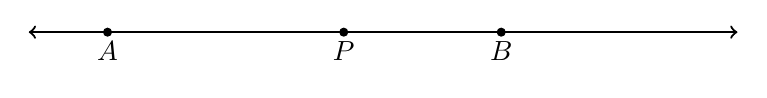
\begin{tikzpicture}
        \draw [<->, thick] (0,0)--(9,0);
        \draw [fill] (1,0) circle [radius=0.05] node[below]{$A$};
        \draw [fill] (6,0) circle [radius=0.05] node[below]{$B$};
        \draw [fill] (4,0) circle [radius=0.05] node[below]{$P$};
      \end{tikzpicture}
      \end{center} \vspace{4cm}
    
\end{enumerate}
\end{document}